 \documentclass[12pt,relax]{TrilinosDevGuide}
\usepackage{array}
    \title{Trilinos Developers Guide}
\SANDsubtitle{}

\author{
Michael A. Heroux \\
James M. Willenbring\\
Computational Mathematics \& Algorithms \\
Robert Heaphy \\
Discrete Algorithms and Math Department \\
Sandia National Laboratories\\
P.O. Box 5800\\
Albuquerque, NM 87185-1110 \\
maherou@sandia.gov \\
jmwille@sandia.gov \\
rheaph@sandia.gov \\
}

    % There is a "Printed" date on the title page of a SAND report, so
    % the generic \date should generally be empty.
    \date{\today} % Remove ``\today'' in final version


\SANDnum{SAND2003-xxxx}
\SANDprintDate{April 2003}
\SANDauthor{
Michael A. Heroux, James M. Willenbring, Robert Heaphy, 
Sandia National Laboratories}


\SANDreleaseType{Unlimited Release}


\SANDdistcategory{UC-999}    

\begin{document}
\maketitle

\begin{abstract}

The Trilinos Project is an effort to facilitate the design, development,
integration and ongoing support of mathematical software libraries.
A new software capability is introduced into Trilinos as a {\it
package}.  A Trilinos package is an integral unit usually developed by
a small team of experts in a particular algorithms area such as
algebraic preconditioners, nonlinear solvers, etc.

The Trilinos Developers Guide is a resource for new and existing
Trilinos package developers.  Topics covered include how to configure and 
build Trilinos, what is required to integrate an existing package into Trilinos
and examples of how those requirements can be met, as well as what
tools and services are 
available to Trilinos packages.  Also discussed are some common practices that 
are followed by many Trilinos package developers.  Finally, a snapshot
of current Trilinos packages and their interoperability status
is provided, along with a list of supported computer platforms.

\end{abstract}


\section*{Acknowledgement}
The authors would like to acknowledge the support of the ASCI and LDRD 
programs that funded development of Trilinos and recognize all Trilinos 
contributors: Teri Barth, Ross Bartlett, David Day, Bob Heaphy, 
Robert Hoekstra, Jonathan Hu, Tammy Kolda, Richard Lehoucq, Kevin
Long, Eric Phipps, 
Roger Pawlowski, Andrew Rothfuss, Andrew Salinger, Paul Sery, Ken
Stanley, Heidi Thornquist, Ray Tuminaro and Alan Williams.

\clearpage
\tableofcontents
\listoffigures
\listoftables

\clearpage

\section*{Nomenclature}
\addcontentsline{toc}{section}{Nomenclature}
\begin{itemize}

\item[Package]
A collection of software focused on one primary class of numerical
methods.  Also a fundamental, integral unit in the Trilinos framework.

\item[Trilinos]
The name of the project.  Also a Greek term which,
loosely translated means ``a string of pearls,'' 
meant to evoke an image that each Trilinos package is a pearl in its 
own right, but is even more valuable when combined with other 
packages.

\item[new\_package] A sample Trilinos package containing all of the
infrastructure to install a new package into the Trilinos framework.
Contains the basic directory structure, a collection of sample
configuration and build files and a sample ``Hello World'' package.

\item[Anasazi]
An extensible and interoperable framework for large-scale eigenvalue
algorithms.The motivation for this framework is to provide a generic
interface to a collection of algorithms for solving large-scale 
eigenvalue problems.

\item[AztecOO] 
Linear solver package based on preconditioned Krylov methods.  A 
follow-on to the Aztec solver package~\cite{Aztec2.1}.  
Supports all Aztec 
interfaces and functionality, but also provides significant new 
functionality.

\item[Belos] A Greek term meaning ``arrow.'' Belos is the next
generation of iterative solvers.  Belos solvers are written using
``generic'' programming techniques.  In other words, Belos is written
using TSF abstract interfaces and therefore has no explicit dependence
on any concrete linear algebra library.  Instead, Belos solvers can be
used with any concrete linear algebra library that implements the TSF
abstract interfaces. 

\item[Ifpack] 
Object-oriented algebraic preconditioner, compatible with 
Epetra and AztecOO.  Supports construction and use of parallel
distributed memory preconditioners such as overlapping Schwarz domain
decomposition, Jacobi scaling and local Gauss-Seidel relaxations.

\item[Komplex] 
Complex linear equation solver using equivalent real 
formulations~\cite{DayHero2000}, built on top of Epetra and AztecOO.

\item[Meros]
Segregated preconditioning package.  Provides scalable block
preconditioning for problems that coupled simultaneous solution
variables such as Navier-Stokes problems.

\item[ML]
Algebraic multi-level preconditioner package.  Provides scalable
preconditioning capabilities for a variety of problem classes.

\item[NOX]
A collection of nonlinear solvers, designed to be easily integrated
into an application and used with many different linear solvers.

\item[Petra]
A Greek term meaning ``foundation.''  Trilinos has three Petra 
libraries: Epetra, Tpetra and Jpetra that provide basic classes 
for constructing and manipulating matrix, graph and vector
objects.  Epetra is the current production version that is
split into two packages, one core and one extensions.

\item[TSF]
Composed of several packages.  TSFCore provides 
a basic collection of abstract interfaces to vectors, linear
operators, solvers, etc.  These interfaces provide a common
interface for applications to access one or more packages that
implement the abstract interface.  These interfaces can also be used
by other packages in Trilinos to accomplish the same purpose.
TSF Extended builds on top of TSFCore, providing implicit
aggregation capabilities and overloaded operators.

\end{itemize}


\section{Introduction}
\label{Section:Introduction}
The Trilinos Project is an effort to facilitate the design, development,
integration and ongoing support of mathematical software libraries.  Trilinos 
provides a framework and set of tools for document and source code control,
software issue tracking, developer and user communication, automatic
testing, portable configuration and building, and software
distribution.  Trilinos also provides a set of core utility libraries
that provide common vector, graph and matrix capabilities, as well as
a common abstract interface for applications to access any appropriate
Trilinos package.

A new software capability is introduced into Trilinos as a {\it
package}.  A Trilinos package is an integral unit usually developed by
a small team of experts in a particular algorithms area such as
algebraic preconditioners, nonlinear solvers, etc.

The overall objective of Trilinos is to promote rapid development and
deployment of high-quality, state-of-the-art mathematical software in
an environment that supports interoperability of packages while
preserving package independence.  The Trilinos design allows 
individual packages to grow and mature autonomously to the extent the 
algorithms and package developers dictate. 

The Trilinos Developers Guide is meant to assist new and existing
Trilinos package developers.  Topics covered include how to configure and 
build Trilinos, what is required to integrate an existing package into Trilinos
and examples of how those requirements can be met, as well as what
tools and services are 
available to Trilinos packages.  Also discussed are some common practices that 
are followed by many Trilinos package developers.  Finally, a snapshot
of current Trilinos packages and their interoperability status
is provided, along with a list of supported computer platforms.

For a higher-level view of the Trilinos project, please see An Overview
of the Trilinos Project~\cite{Trilinos-Overview}. The current set of
packages in Trilinos is shown in Figure~\ref{Figure:TrilinosPackages}.

\begin{figure}
%\begin{center}
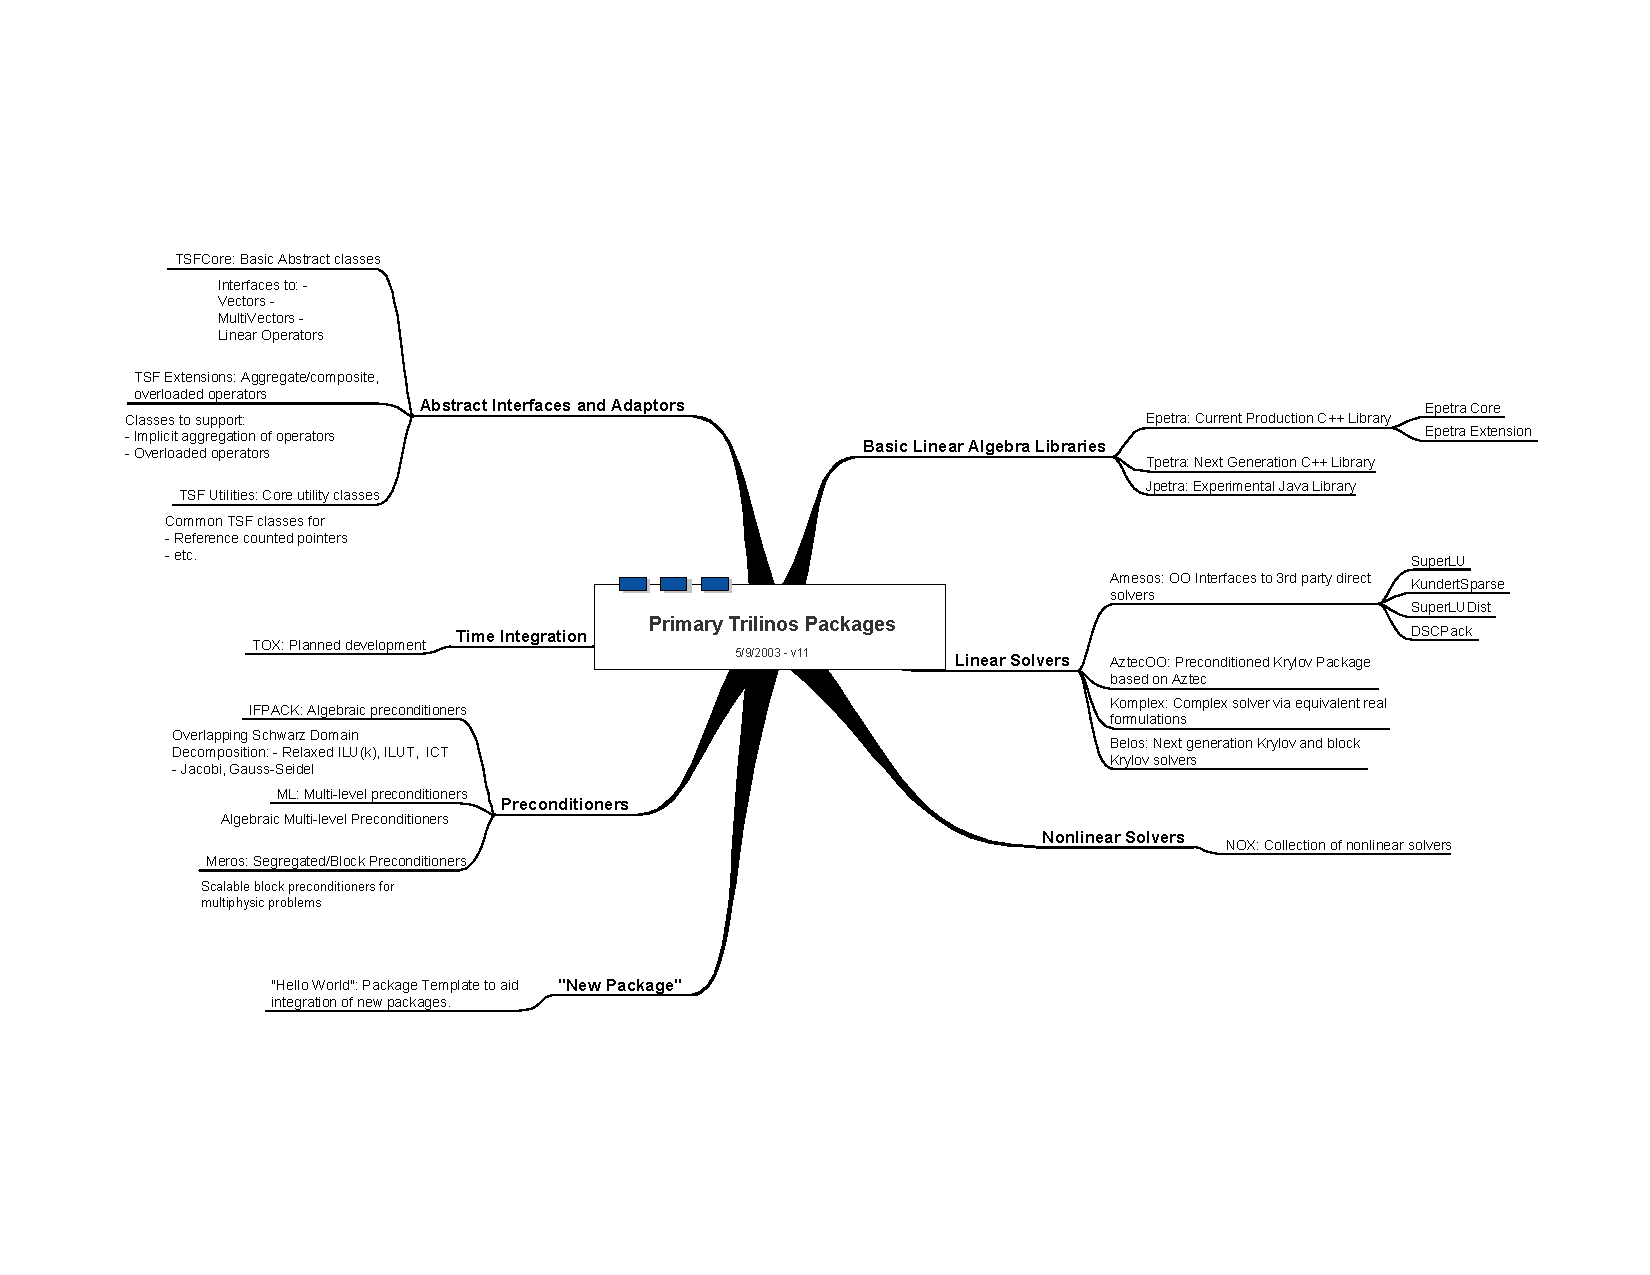
\includegraphics[height=8in]{TrilinosPackagesDiagram}
%\end{center}
\label{Figure:TrilinosPackages}
\caption{Current collection of Trilinos Packages}
\end{figure}

\subsection{How To Use This Guide}

Although all sections of this guide will be useful to most developers,
it is worth mentioning that 
this guide supports three types of development activities:
\begin{enumerate}
\item New Project: Development of a new package using little or no
existing software as a base.  All sections of this guide are
appropriate reading.
\item Integration of an existing third-party software: In this case,
existing software is being imported into the Trilinos framework.  In
this case, Section~\ref{Section:IntegratingPackages} is particularly
important, as are Sections~\ref{Section:AvailableServices},
~\ref{Section:PackageRequirements} and~\ref{Section:EpetraAndTSF}.
\item Ongoing development:  For existing Trilinos package developers,
Sections~\ref{Section:AvailableServices}
and~\ref{Section:PackageRequirements} are designed as a reference for
software engineering practices and policies for Trilinos development.
\end{enumerate}

\subsection{Typographical Conventions}

Our typographical conventions are found in
Table~\ref{Table:TypoConventions}.
\begin{table}[ht]
\scriptsize
\begin{center}
\begin{tabular}{|l|l|p{2.0in}|} \hline
Notation & Example & Description \\ \hline
\InlineCommand{Verbatim text} & \InlineCommand{../configure --enable-mpi} & 
Commands, directory and file name examples, and other text associated
with text displayed in a computer terminal window. \\ \hline
\InlineCommand{CAPITALIZED\_TEXT} & \InlineCommand{CXXFLAGS} & 
Environment variables used to configure how tools such as compilers behave. \\ \hline
\InlineCommand{[text in angle brackets]} & \InlineCommand{../configure
<user parameters>} & 
Optional parameters. \\ \hline
\end{tabular}
\end{center}
\caption{\label{Table:TypoConventions} Typographical Conventions for This Document.}

\end{table}


\section{Getting Started}
\label{Section:GettingStarted}
This chapter covers some of the basics that a developer will need to know when 
beginning to work on the Trilinos project.  We address how to configure and 
build Trilinos, as well as how to add files to an existing package.

\subsection{Recommended Build Directory Structure}

Via Autoconf and Automake the Trilinos configuration facilities
provide a great deal of flexibility for configuring and building the
existing Trilinos packages.  However, unless you have prior experience
with Autotools, we recommend the following process to build and
maintain your local builds of Trilinos.

To start, we defined two useful terms:
\begin{itemize}
\item Source tree - The directory structure where source files are found.  A source 
tree is obtained by expanding a distribution tar ball, or by checking 
out a copy of the Trilinos repository.  
\item Build tree - The directory structure where object and library files, as well 
as executables are located.  
\end{itemize}
 
\begin{minipage}[c]{\textwidth}

\begin{minipage}[l]{.6\textwidth}

Although it is possible to run \InlineCommand{./configure} from the source tree (in 
the directory where the configure file is located), we recommend that a 
user have separate build trees.  The greatest advantage to having a separate 
build tree is that multiple builds of the libraries can be maintained
from the same source tree, for 
example, serial and parallel libraries.  A less obvious advantage is that 
this approach eliminates problems with configuring in a 'dirty'
directory (one that has 
already been configured in).
\end{minipage}\hfill
\framebox{\begin{minipage}[r]{.35\textwidth}{
{\bf Key Point:}
$\ldots$ we recommend that a 
user have separate build trees $\ldots$ multiple builds of the
libraries can be maintained from the same source tree $\ldots$ 
eliminates problems with configuring in a 'dirty'
directory $\ldots$
}\end{minipage}}
\end{minipage}

Setting up a build tree is straight-forward.
Figure~\ref{Figure:TrilinosDirectoryStructure} illustrates the
\begin{figure}
\begin{center}
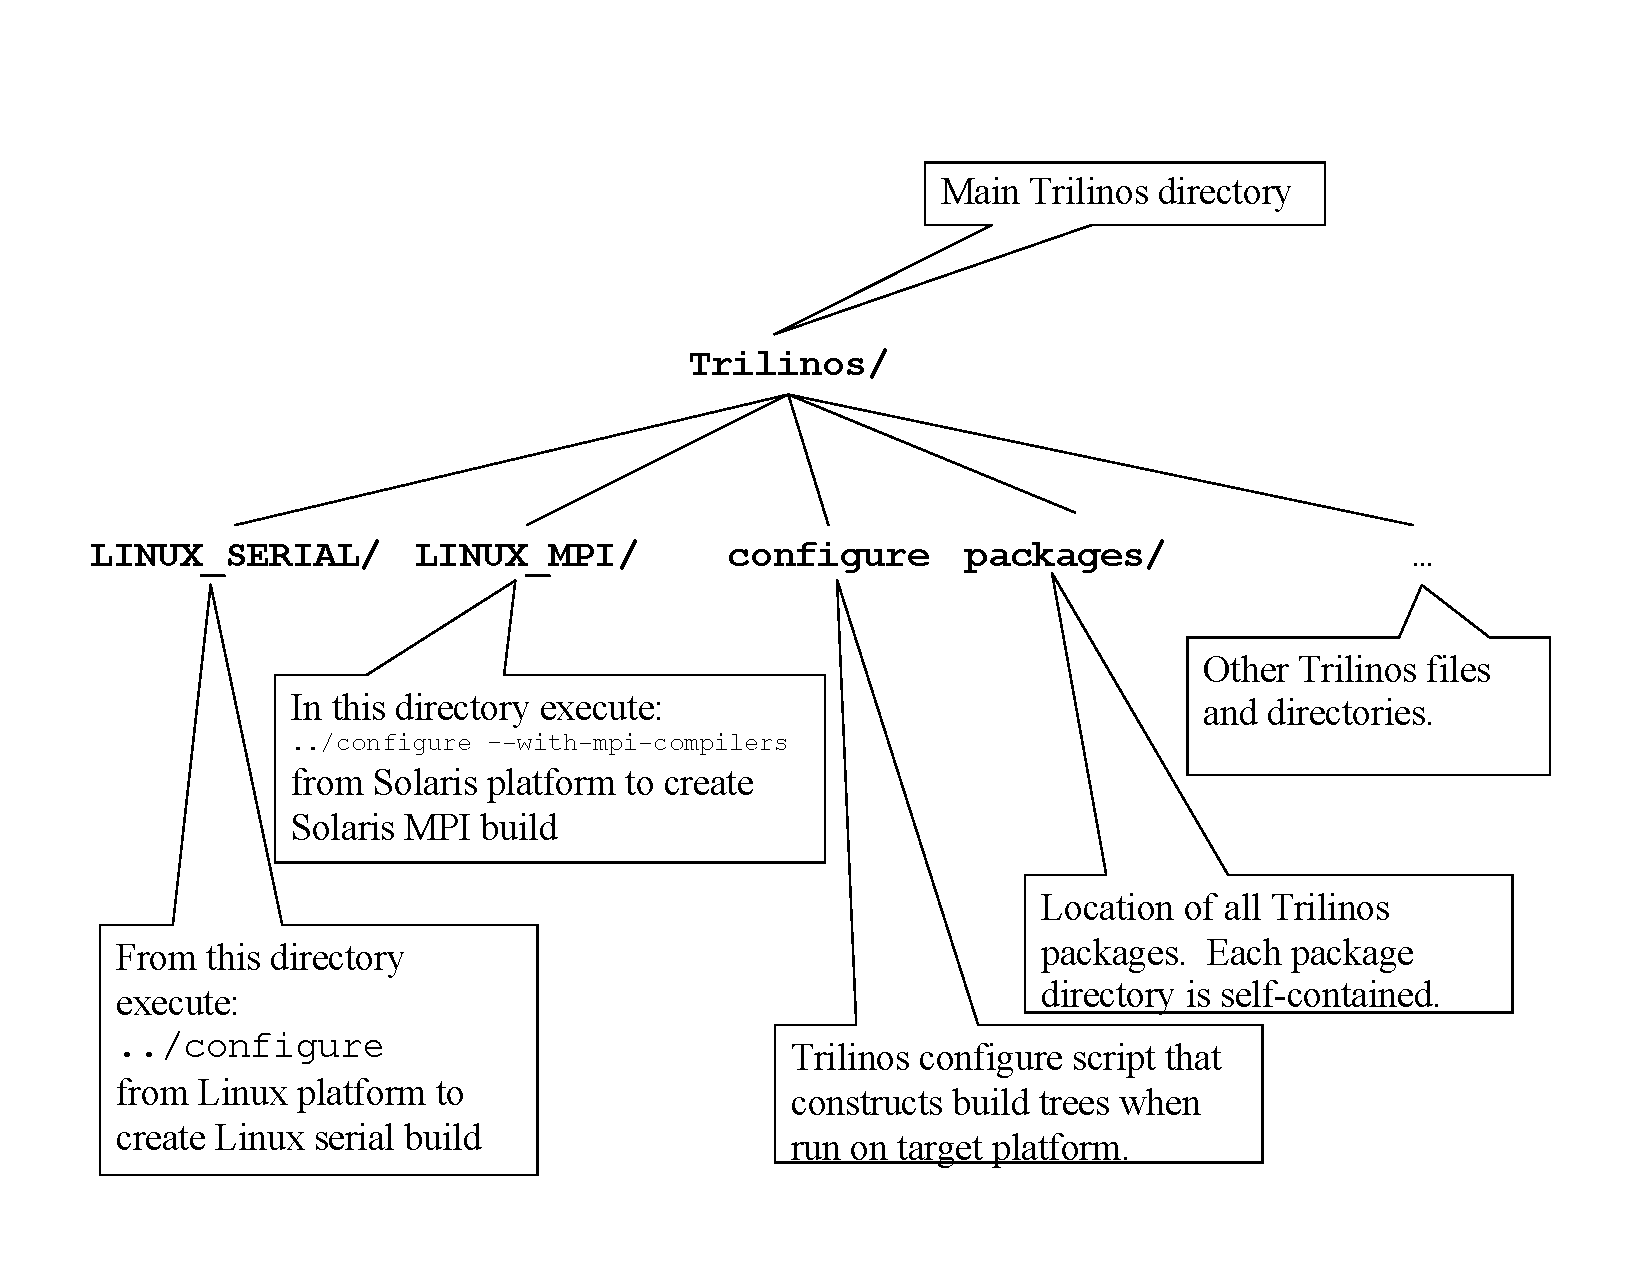
\includegraphics[width=4in]{TrilinosDirectoryStructure}
\end{center}
\label{Figure:TrilinosDirectoryStructure}
\caption{Recommended Layout for Trilinos Build Directories}
\end{figure}recommended layout.  First, from the highest 
directory in the source tree (Trilinos for a repository copy, Trilinos-3.0.1 
for a distribution), make a new directory - for an MPI build
on a Linux platform, a 
typical name could be \InlineDirectory{LINUX\_MPI}.  
Finally, from the new dirctory, type

\DisplayCommand{../configure --with-mpi-compilers}

(Note that various configure options might be necessary, see Section~\ref{Subsection:ConfiguringTrilinos} for details.)  Finally, type

\DisplayCommand{make}


In summary:

\begin{verbatim}
       cd Trilinos
       mkdir LINUX_MPI
       cd LINUX_MPI
       ../configure --with-mpi-compilers
       make
\end{verbatim}
At this point, the MPI version of Trilinos on a Linux platform is
built and completely contained in the \InlineDirectory{LINUX\_MPI}
directory.  No files outside this directory have been modified.  This
procedure can be repeated for any number of build targets.

{\bf Note:} Although we recommend the above location for build trees,
they can be set up anywhere.

\subsection{Configuring Trilinos}
\label{Subsection:ConfiguringTrilinos}
	To configure from a remote build tree, simply run the configure script 
in source tree from the root of the build tree.  In the example above, cd to 
the SOLARIS\_SERIAL directory and type 
\DisplayCommand{../configure <options as described below>}

A detailed list of configure options can be seen by typing
\DisplayCommand{./configure --help=recursive} from the top level of the 
source tree.  This will display the help page for the Trilinos level as well as all 
Trilinos packages that use autoconf and automake.  The output from this command
is quite extensive.  To view the help page for an individual package, cd to 
the home directory for the package in the source tree and type 
\DisplayCommand{./configure --help} 
This command will also display the help page for Trilinos level 
options when used from the Trilinos home directory in the source tree.


	The user needs to provide two important pieces of information at this 
stage.  First, the user needs to describe what kind of a build is needed.  For 
instance, serial or mpi, all of the packages, or just a proper subset.  

	For example, to configure for serial libraries, no action is necessary,
but to configure for parallel libraries, a user must append appropriate 
arguments to the configure invocation line as described in ``Trilinos 
Configuration Options'', section~\ref{subsect:TrilinosConfigOptions}.

	Also, to build the default set of Trilinos libraries, no action is 
necessary, but to exclude a default package, komplex for example, a user must 
append \InlineCommand{--disable-komplex} to the configure invocation  line.  
Similarly, to include a package that is not currently built by default, NOX 
for example, users must append \InlineCommand{--enable-nox} to the configure 
invocation line.  It is recommended that users always configure from the 
Trilinos level and use \InlineCommand{--disable-<package>} as necessary, 
rather than trying to configure from a lower level.  To see which packages 
build by default and which ones don't, simply cd to the Trilinos home 
directory and type \DisplayCommand{./configure --help}


{\bf NOTES:} 
\begin{enumerate}
\item {\bf Ifpack versions:} 
Ifpack is divided into old and new versions.  Future ifpack developments 
will replace all of old ifpack, but at this time some users will need to append
\InlineCommand{--enable-oldifpack} to the configure line.

\item {\bf Enabling/Disabling package builds:} 
The configure process is set up to detect when a 
\InlineCommand{--disable-<package>} option would break a package dependency.  
For example, ifpack depends on epetra, so if a user wants to build ifpack, but 
types \InlineCommand{--disable-epetra}, epetra will be configured and built 
anyway.  However, some of the tests and examples have different dependencies 
than the core package.  It is possible that not all of these dependencies have 
been accounted for.  Please submit a bug report for any problems found with 
this matter.

\item {\bf Installing libraries and header files:}
To install libraries and header files in a particular location, 
use \InlineCommand{--prefix=<dir>} on the configure line.  If this option is 
used, libraries will be located in \InlineDirectory{<dir>/lib} and header files in 
\InlineDirectory{<dir>/include/<package>}.

\item {\bf Providing additional information to autotools:}
Although autotools will attempt to determine all configuration
information on its own, in some situations the user must provide 
the name or location, or both, of anything that autotools needs and 
cannot find on its own.  Also, if autotools selects, for example, the wrong 
BLAS library by default, the user must indicate which blas library to use.  
Other more obscure issues dealing with topics such as standards 
non-compliance are also dealt with here.  If all required libraries (often 
BLAS, and LAPACK) are located in standard places, try configuring with what 
you have.

\item {\bf Sample configure invocation scripts:}
For a machine that requires additional configure line options, a good 
place to look for examples is \InlineDirectory{Trilinos/config}.  There are 
configure invocation scripts here for various platforms.  These scripts are 
named using the following naming convention:
\InlineCommand{arch\_comm\_machine}.
For example \InlineCommand{sgi64\_mpi\_atlantis}.  Note that these scripts are 
examples only.  Users should not necessarily expect to be able to find the 
perfect script and use it, but rather should choose a script for a similar 
machine, examine the options used in the script and figure out if those 
options make sense for the case at hand.  Some of the scripts in the 
repository are not always up to date.  If a user submits a script for a 
machine that few Trilinos developers have an account on, that script may 
become obsolete if it is not updated by the user who submitted it.  Therefore, 
these scripts are primarily useful for the values of options such as 
\InlineCommand{LDFLAGS}, \InlineCommand{CPPFLAGS}, 
and \InlineCommand{CXXFLAGS}.  

Users who create scripts for other machines are encouraged to check them into 
the repository for the benefit of other users.  Users who do not have access to
the repository can send their scripts to \InlineCommand{jmwille@sandia.gov}.
\end{enumerate}

\subsection{Building Trilinos}

If the configure stage completed successfully, just type \DisplayCommand{make}
 and if 
\InlineCommand{--prefix} was specified, \DisplayCommand{make install}

The following section describes the configuration options mentioned above that 
are common to all Trilinos packages.  These options DO NOT cover all options 
for all Trilinos packages.

\subsection{Trilinos Configuration Options}
\label{subsect:TrilinosConfigOptions}
The following options apply to all Trilinos packages unless 
the option doesn't make sense for a particular package (for example, a 
package that does not include any Fortran code will not be sensitive to 
\InlineCommand{F77=g77}), or otherwise noted.  For options specific to 
individual package, cd to the home directory of the source code of the 
individual package and type \DisplayCommand{./configure --help}.

Basic Options

\begin{itemize}
\item \InlineCommand{--enable-debug} 

(Nox only.)  This turns on compiler debugger flags. It has 
not been fully tested. As an alternate, specify CXXFLAGS on the 
                 configure line.

\item \InlineCommand{--enable-opt}

(Nox only.)  This turns on compiler optimization flags. It 
has not been fully tested. As an alternate, specify CXXFLAGS on the 
                 configure line. 

\item \InlineCommand{--with-cppflags}

Specify additional preprocessor flags (e.g., "-Dflag -Idir") 

\item \InlineCommand{--with-cxxflags}

Specify additional C++ flags 

\item \InlineCommand{--with-ldflags}

Specify additional linker flags (e.g., "-Ldir") 

\item \InlineCommand{--with-ar}

Specify a special archiver command, the default is "ar cru". 
\end{itemize}

 Influential Environmental Variables

\begin{itemize}
\item \InlineCommand{CC}

C compiler command.

\item \InlineCommand{CFLAGS}

C compiler flags.

\item \InlineCommand{CXX}

C++ compiler command.

\item \InlineCommand{CXXFLAGS}

C++ compiler flags.

\item \InlineCommand{LDFLAGS}

Specify linker flags.

\item \InlineCommand{CPPFLAGS}

C/C++ preprocessor flags.

\item \InlineCommand{CXXCPP}

C++ preprocessor.

\item \InlineCommand{F77}

Fortran 77 compiler command.

\item \InlineCommand{FFLAGS}

Fortran 77 compiler flags.
\end{itemize}

MPI-Related Options

\begin{itemize}
\item \InlineCommand{--enable-mpi}

Enables MPI mode. Defines HAVE\_MPI in the (Package)\_Config.h file. Will test 
for the ability to preprocess the MPI header file and may test ability to link 
with MPI.  This option is rarely necessary as many of the below options also 
turn MPI on.  

\item \InlineCommand{--with-mpi-compilers}

Sets CXX = mpicxx (or mpiCC if mpicxx not available), the CC = mpicc and 
F77 = mpif77.  Automatically enables MPI mode.  To use compilers other than 
these, specify mpi locations with the below options.  If none of these options 
are necessary, don't forget to use \InlineCommand{--enable-mpi}.  In this 
case, CXX, CC, and F77 may also have to be set if the correct compilers are 
not chosen by default.

\item \InlineCommand{--with-mpi=MPIROOT}

Specify the MPI root directory. Automatically enables MPI mode.  If this 
option is set, \InlineCommand{--with-mpi-incdir} and 
\InlineCommand{--with-mpi-libdir} should not be used.  
\InlineCommand{--with-mpi} is meant to be a shortcut for setting \newline
\InlineCommand{--with-mpi-libdir=MPIROOT/lib} 
and \InlineCommand{--with-mpi-incdir=MPIROOT/include}.  Use these two options instead if 
these default locations are not correct.

\item \InlineCommand{--with-mpi-libdir=DIR}

Specify the MPI libraries location. Defaults to MPIROOT/lib if 
\InlineCommand{--with-mpi} is specified. If multiple directories must be 
specified, try \newline
\InlineCommand{--with-ldflags="-L<dir1> -L<dir2>"} instead. 

\item \InlineCommand{--with-mpi-libs="LIBS"} 

Specify the MPI libraries. Defaults to \InlineCommand{"-lmpi"}
 if either\InlineCommand{ --with-mpi} or 
\InlineCommand{--with-mpi-libdir} is specified.

\item \InlineCommand{--with-mpi-incdir=DIR}

Specify the MPI include files location. Defaults to \InlineDirectory{MPIROOT/include} if 
\InlineCommand{--with-mpi} is specified. If multiple directories  must be specified, try 
\newline
\InlineCommand{--with-cppflags="-I<dir1> -I<dir2>"} instead.
\end{itemize}

Developer-Related Options
\begin{itemize}
\item \InlineCommand{--enable-maintainer-mode}

Enable make rules and dependencies not useful (and sometimes confusing) to 
the casual installer.
\end{itemize}

Other important notes about the configure and build processes.
\begin{itemize}
\item Any code that links to Trilinos should define 
\InlineCommand{HAVE\_CONFIG\_H}.

\item Often the output from configure will be inadequate for diagnosing 
problems.  A developer should look (in the buildtree) at the config.log file 
for the package that failed to configure properly.  To figure out which 
package failed to configure, simply look at the bottom of the output from the 
\InlineCommand{configure} command.  One of the last lines should say something 
like:

\begin{verbatim}
    configure: error: /bin/sh '../../../packages/epetra/configure' 
    failed for packages/epetra.
\end{verbatim}

This particular error indicates to look in 
\InlineDirectory{packages/epetra/config.log}.  This file is useful for 
developers trying to build Trilinos, and those who are 
adding or editing autoconf-specific files such as configure.ac.

\item The ``classic'' build system and Autotools do not mix.  Trying to build 
with Autotools in a directory that contains a classic build will not work.  
Before attempting an autotools build, the classic build object, library, and 
executable files within the source tree should be removed.
\end{itemize}

\subsection{Adding and Removing Source Files}
\label{Subsection:AddSource}
%add how to add directories
Commonly a developer needs to add files to or remove files from a Trilinos 
package.  We outline the steps for adding or removing source files from a 
Trilinos package that uses Autotools.  The below outline assumes the simple 
addition or removal of files.  Special situations such as adding header file 
or library dependencies to a Trilinos package or conditionally compiling new 
files require a more complicated process.  In addition, the following 
restrictions apply only to development and release branches.  If a branch is 
established for a separate purpose (for example, to attempt an experimental 
restructuring of existing code), the restrictions do not apply.  However, in 
this case, the restrictions do apply when any changes from the branch are to 
be merged back into the development branch.
 
\begin{enumerate}
\item Obtain the supported versions of Autoconf and Automake.

The current supported versions of Autoconf and Automake are documented in 
the Trilinos repository.  
\InlineDirectory{Trilinos/config/AutotoolsVersionInfo} contains the 
information.  The Trilinos team does not attempt to keep up with the latest 
versions of Autoconf and Automake, so please do not assume that the most 
recent versions are supported.  The supported versions of Autoconf and 
Automake can always be found on software.sandia.gov.  This makes software a 
good machine to bootstrap on.  However, software does not currently have an
mpi implementation installed.

\item Update source code from Trilinos repository

Obtain the most current version of Trilinos (for the branch being worked on).  
From the top Trilinos directory type

\DisplayCommand{cvs -q update -dP}

\item Add new files to or remove obsolete files from the Trilinos repository

To add new files abc.cpp and abc.h to the Trilinos repository, type

\DisplayCommand{cvs add abc.cpp abc.h}

in the directory where the files are located (in a checked out version of the 
Trilinos repository).  To remove the same files, type

\DisplayCommand{cvs remove abc.cpp abc.h}

The above commands do not actually add the files to or remove the files from 
the repository, but simply prepare for the addition or removal of the files.  
The initial version of the file will be added to the repository later using 
\InlineCommand{cvs commit}.  However, this is a necessary step in the process.

\item List new files in or remove obsolete files from Makefile.am

New source files should be placed into a category in the appropriate 
Makefile.am.  Typically, the directory in which the new files are located will 
contain a Makefile.am.  If not, the appropriate Makefile.am will be found in 
the Makefile.am that is in the parent directory directly above the directory 
in which the new files are located.  The number of possibly categories to add 
files to varies a lot.  For a test or example a developer will typically just 
add the files directly to a SOURCES primary.  For a Trilinos package, there 
may be several categores of files.  For example UTIL, CORE, and DIST, to name 
a few.  Do not worry too much about which macro category to add the files to.  
The categories are simply a way to sort files into logical groups.  To remove 
files from the build process, simply delete the file names from the 
appropriate Makefile.am.

\item Bootstrap

First, from the top-level directory of the appropriate Trilinos package (for 
example Trilinos/packages/epetra), type 

\DisplayCommand{./bootstrap}

The bootstrap should complete without any errors, but the following warnings 
commonly occur:

\begin{verbatim}
warning: do not use m4_patsubst: use patsubst or m4_bpatsubst
warning: do not use m4_regexp: use regexp or m4_bregexp
\end{verbatim}

\item Test the new code

Reconfigure and rebuild the Trilinos package.  Perform tests associated with 
the new code, as well as the rest of the tests for the package to insure that 
both the new code works and existing code has not been broken.  When changes 
could possibly affect other packages, tests for affected packages should also 
be run.  The simple way to run all of the required tests is to use the 
checkin test harness.  This script can be found in \newline
\InlineDirectory{Trilinos/testharness/checkin-test-harness}.  Directions 
explaining how to run the tests associated with the checkin test harness can 
be found in the comments at the top of the script itself.

\item Update source code from Trilinos repository

Didn't we just do this?  Yes, but there are two good reasons to do it again.

Other developers could have committed changes during the past several 
steps of this process.  Though is not likely, it is worth checking.  If 
changes were committed, minimally the testing step will need to be redone.  
If files related to configuring or building were modified, more will have to 
be done if collisions occur.  Some of the possibilities are beyond the scope 
of this introductory document, however we will briefly discuss the most 
common collision scenario.  Typically the generated files will contain 
collisions (for example configure, Makefile.in, or aclocal.m4), while the 
changes in the files created by developers (for example configure.ac or 
Makefile.am) will be successfully merged by CVS.  In this case, the best 
course of action is to remove the files with collisions, cd to the top level 
of the Trilinos package, perform a \InlineCommand{cvs update}, and then begin 
the above process again from ``Bootstrap'' step.  As long as the changes are 
merged in the non-generated files, bootstrapping should resolve the problem.

An even better reason to update again before committing changes is to avoid 
confusion.  After a bootstrap, all of the generated files will get an updated 
timestamp, but in most cases only some of the files will actually be 
modified.  If a developer commits changes before updating, all of the 
generated files will be viewed as having been modified.  This is bad for 
several reasons.  One of the most important is that when committing changes, a 
developer should always verify that the list of files that are about to be 
committed makes sense.  The list is guaranteed to not make sense if files are 
going to be committed that have not been changed.  A cvs update will check to 
see if the file has really been changed or if it simply has a new timestamp.

\item Commit the changes to the Trilinos repository

Once all of the above steps are completed, the final step is to commit the 
changes to the repository.  Start by typing

\DisplayCommand{cvs commit}

Now, look at the list of files that are to be added, removed  or modified.  
It is easy to inadvertantly commit files.  It is also easy to forget to use 
\InlineCommand{cvs add}.  If a file has not been added, it will not show up on 
the list of files to be added.  Conversely, to remove a file, don't forget to 
use \InlineCommand{cvs remove}.  

Here are a few helpful tips to use when verifying the list of files 
to be committed.  First, make sure that all files you modified directly appear 
in the list.  Second, when modifying a Makefile.am, the corresponding 
Makefile.in will change also.  Third, when modifying configure.ac, configure 
will also change, but some Makefile.in files may also change when using macros 
such as AC\_SUBST.  Finally, when unsure about whether or not a 
file should be in the commit list, abort the commit by closing the edior 
without saving, and chosing \InlineCommand{abort}.  Then, if abc.cpp is in 
question, type 

\DisplayCommand{cvs diff abc.cpp}

Then look at the diff output and see if it makes sense for the changes that 
were made.  After verifying that all of the files that are in the list belong 
there, and that all files that belong in the list are, in fact, listed, remove 
unnecessary instances of ``CVS: `` from the log message and enter an 
appropriate description of the changes that are to be committed.  Don't forget 
to reference any appropriate Bugzilla bug numbers.  Further, detailed log 
messages make it easier to track problems in the future.  It is a good habit 
to indicate which tests were run before making the change.

Finally, save the file, and exit the CVS editor to commit the changes.

When using the above process to commit new source code, the new source must 
be functioning properly, otherwise the repository will not be stable.  
At the same time, developers are encouraged put new code into the repository 
during initial development.  This will ensure that work is backed up and 
provide version control.  When adding unstable code to the repository, only
two steps are necessary.  First, use the \InlineCommand{cvs add} command as 
mentioned above, and then modify the commit command slightly to commit only 
the new source by typing

\DisplayCommand{cvs commit newfile1.cpp newfile2.cpp}

Provided that the new files are not added to the make structure, the addition 
of the new files should not negatively affect the repository.  Distribution 
tarballs will even skip over the new source.  A common log message for this 
type of commit is simply ``Checking in for safe keeping; code is not yet 
funcitoning''.  Sometimes developers will include a short description of what 
the code will do when complete.
\end{enumerate}

\section{Services Available to Trilinos Packages}
\label{Section:AvailableServices}
A number of services exist for Trilinos packages.  Many of these services 
relate directly to the requirements and suggested practices for Trilinos 
packages.  For example, the CVS repository is discussed below, and 
Trilinos packages must make use of this repository.  Also, Bonsai, Bugzilla 
and Mailman are all tools that relate to suggested practices.  (It should be 
noted that these services are not simply meant to satisfy SQE requirements.  
Rather, Bonsai, Bugzilla and Mailman have proved to be very useful tools.  
Using these tools together, along with the CVS repository, has led to a more 
time and cost effective code development process.)  For more information about 
any of the below services, please contact the Trilinos Project Leader.

\subsection{Configuration Management}
Autoconf~\cite{Autoconf},  Automake~\cite{Automake} and Libtool~\cite{Libtool} 
provide a robust, full-featured set of tools for building software across a 
broad set of platforms (see also the ``Goat Book''~\cite{GoatBook}).  Although 
these tools are not official standards, they are commonly used in many 
packages.  Many existing Trilinos packages use Autoconf and Automake (and will 
use Libtool in the future).  However, use of these tools is not required.

Package developers who are not currently using autotools, but would like
to, can get a jump start by using a Trilinos package called 
``new\_package''.  This trivial package exists for one primary purpose.  
It walks a developer through the process of setting up a package to 
configure and build using autotools.  General instructions for how to get 
started can be found in Section~\ref{Section:IntegratingPackages}.  Please 
note that new\_package is a work in progess, suggestions and contributions are 
welcome, especially for FAQ's.

Trilinos provides a set of M4~\cite{M4} macros that can be used by any other
package when its Autoconf and Automake configure and build system is being 
setup.  These macros perform common configuration tasks such as
locating a valid LAPACK~\cite{lapack} library, or checking for a user-
defined MPI C compiler.  The macros can be found in the Trilinos CVS 
repository in Trilinos/config.  These macros minimize the amount of redudant
 effort in using Autotools, and make it easier to apply a general change to 
the configure process for all packages.
\subsection{Regression Testing}
Trilinos provides a variety of regression
testing capabilities.  Within a number of Trilinos packages, we employ
``white box'' testing where detailed information about the software is
used and probed.  In the future, Trilinos will perform ``black box'' testing
of packages via the Trilinos Solver Framework (TSF) virtual class
interfaces.  Any package that implements the TSF interfaces (see
Section~\ref{subsect:InteropTSF} below) will be tested via this black box
test environment.

\subsection{Test Harness}
\label{subsect:TestHarness}

Trilinos packages that configure and build using Autotools can easily 
utilize the the Trilinos test harness.  The Trilinos test harness is composed 
of two components.  

One part of the test harness is used to run nightly tests on a number of 
platforms.  This portion of the test harness performs a 
\InlineCommand{cvs update} (gets the most recent source code) every night and 
then builds the libraries and runs any tests that have been integrated into 
the test harness.  

Tests that are added as ``daily'' tests are run six time a week, while 
``weekly'' tests are run once a week.  Currently the nightly test harness only 
runs on Linux, IRIX64, and DEC/OSF1, but it will eventually run on 5-8 
platforms.  Packages that have not ported to a particular platform can be 
excluded from the testing process on that platform.  Packages that do not have 
any tests integrated into the test harness can still benefit by testing that 
libraries build without errors.  

The second component of the test harness is a script that should be executed 
by users before checking updates into the repository.  This script is located 
in \InlineDirectory{Trilinos/testharness/checkin-test-harness}.  The script 
provides an easy way for users to run all of the ``daily'' tests that have 
been added to the test harness for all packages from one location.  
Instructions for running the script can be found within the script itself.

Integrating existing tests into the testharness is not difficult.  
The process is discussed in 
\InlineDirectory{Trilinos/testharness/HowToAddToTestHarness}.  
Please note that this document is a work in progress.

\subsection{CVS Repository}

Trilinos source code is maintained in a CVS~\cite{CVS} repository.  It is 
very easy to add new packages to the repository.  Packages that already use 
CVS can even retain their CVS history!  To access the repository, one must 
have an account on software.sandia.gov.  Once an account has been granted, 
set the following two environment variables (replace ``your\_user\_name'' 
with your user name on software):

\DisplayCommand{CVSROOT :ext:your\_user\_name@software.sandia.gov:/space/CVS}
\DisplayCommand{CVS\_RSH ssh}

For those not familiar with CVS, a brief discussion covering some of the most 
common CVS commands is available in~\ref{Section:CVS}.  For a more complete 
listing of CVS commands, see the Gnu CVS Home Page~\cite{CVS}.

\subsection{Bonsai}
A lot of useful information related to CVS history is accessible via a
web-based interface package called Bonsai~\cite{Bonsai}.  This tool can be 
found on the web at 
\newline
\InlineDirectory{http://software.sandia.gov/bonsai}.  Bonsai gives a 
developer the ability to view the changes made to the files in the 
repository.  The tool can be especially useful when trying to figure out which 
changes may have introduced bugs into a piece of code.  Developers can search 
for changes based on filename, directory, branch, date, user who made the 
change, or any combination of these criteria.  The entire revision histories of
individual files can be utilized in finding the source of 
bugs.  The differences between any two versions of a file may also be viewed.  

\subsection{Bugzilla}
\label{subsect:Bugzilla}
Feature and issue reports are tracked using Bugzilla~\cite{Bugzilla}.  
Bugzilla can be found on the web at 
\InlineDirectory{http://software.sandia.gov/bugzilla}.  
A Bugzilla account is necessary for submitting bugs.  Those interested can 
sign up at the website.  All bugs related to any package of Trilnos that uses 
Bugzilla should be submitted to Bugzilla.  This even applies to cases in which 
one developer diagnoses and fixes a bug within a short period of time.  A bug 
report is still very valuable in this case because it provides an artifact 
that outlines the problem and explains how the problem was fixed.  A bug 
report should be filled out with as much detail as possible.  Likewise, after 
a bug has been resolved, the developer should also provide a detailed 
description of the solution that was used.

NOTE: In the context of Bugzilla, ``bug'' can refer not only to an error in 
existing code, but also to a desired enhancement.  For example, a bug report 
should be submitted to Bugzilla to report a segmentation fault that occurs 
when using an existing Ifpack preconditioner, and a bug report should also be
submitted to request a new Ifpack preconditioner.  ``Issue'' and ``bug'' are 
used interchangably in the discussion of Bugzilla in this guide.

\subsection{Mailman}
\label{subsect:MailMan}
Email lists are maintained for Trilinos as a whole and for each package 
through Mailman~\cite{Mailman}.  This tool can be found on the web at 
\newline
\InlineDirectory{http://software.sandia.gov/mailman/listinfo}.  
Those interested in signing 
up for one or more lists may do so at the website.  Non-Sandians are able to 
sign up for the ``Users'' and ``Announce'' lists.  Sandians should keep this 
in mind when posting to these lists.

Lists for new packages can be set up very easily.  Each package usually has 
five mailing lists.  The example mailing lists mentioned below are to be used 
for issues relating to all of Trilinos.  The names for the lists pertaining to 
individual packages follow the same naming scheme, simply replace ``Trilinos'' 
with the name of the package.  For example the list for Trilnos users is 
called Trilinos-Users and the email address is 
\InlineCommand{trilinos-users@software.sandia.gov}  The list 
for Epetra users is called Epetra-Users and the associated email address is 
\InlineCommand{epetra-users@software.sandia.gov}

TIP: While those who use Epetra (or any other Trilinos package) are also
``Trilinos users'', the lists are not set up to recognize this.  In other 
words, those who subscribe to the Epetra-Users mailing list do not necessarily 
form a subset of those who subscribe to the Trilinos-Users mailing list.  This 
is also true of all other list types.  Keep this in mind when subscribing and 
posting to lists.
\begin{itemize}
\item Trilinos-Announce 
\InlineCommand{trilinos-announce@software.sandia.gov}

All Trilinos release announcements and other major news.

\item Trilinos-Checkins 
\InlineCommand{trilinos-checkins@software.sandia.gov}

CVS commit log messages that are releated to Trilinos in general or packages 
that have not had separate lists established.

\item Trilinos-Developers 
\InlineCommand{trilinos-developers@software.sandia.gov}

All discussions releated to Trilinos-specific development (not specific to a 
Trilinos package) are conducted via this list.  Important development 
decisions that originate in other places (regular email, discussions, etc) 
should also be posted to this list (or to the appropriate package list).  
By doing this, the list archive can provide a record explaining why various 
changes were made over time.

\item Trilinos-regression 
\InlineCommand{trilinos-regression@software.sandia.gov}

All regression test output that is not specific to a package. 

\item Trilinos-Users 
\InlineCommand{trilinos-users@software.sandia.gov}

List for Trilinos Users.  General discussions about the use of Trilinos.

\item Trilinos-Leaders
\InlineCommand{trilinos-leaders@software.sandia.gov}

Mailing list for representatives for each Trilinos package.  There are no 
leaders lists for individual packages.
\end{itemize}

%**Consider an example showing how tools can work together to fix bugs.**

	\subsection{Portable Interface to BLAS and LAPACK}
%	**(See Overview Doc pg 12)**

Portable interface to BLAS and LAPACK: The Basic Linear Algebra
Subprograms (BLAS)~\cite{BLAS1,BLAS2,BLAS3} and LAPACK~\cite{lapack}
provide a large repository of robust, high-performance mathematical
software for serial and shared memory parallel dense linear algebra
computations.  However, the BLAS and LAPACK interfaces are Fortran
specifications, and the mechanism for calling Fortran interfaces from
C and C++ varies across computing platforms.  Epetra (and Tpetra)
provide a set of simple, portable interfaces to the BLAS and LAPACK
that provide uniform access to the BLAS and LAPACK across a broad
set of platforms.  These interfaces are accessible to
other packages.

\section{Trilinos Package Requirements}
\label{Section:PackageRequirements}
The philosophy of the Trilinos project is to minimize the number of
explicit requirements placed on packages.  Instead, we attempt to
describe high-level requirements coupled with {\it suggested
practices}.  This approach allows freedom to define how
requirements are satisfied yet, at the same time, provides guidance
and support for packages that do not have a full set of established
software engineering practices.  In rare cases, requirements may be waived for 
packages on a case-by-case basis with the approval of the Trilinos Project 
Leader.

Package requirements can be split into two basic categories:
\begin{enumerate}
\item Interoperability mechanisms: Depending what a new Trilinos
package does, it should be able to interact with one or more other
Trilinos packages.  Often this means being able to accept an application
matrix and vector objects as either TSF objects or Epetra objects, and
that the package implements relevant TSF abstract interfaces.
Response to Trilinos configuration options also falls in this category.
\item Software engineering processes: This category includes formal
support for software design, implementation and support, including
processes for capturing user requirements, documenting
design, source control, user documentation, issue tracking and product
release.
\end{enumerate}

Trilinos package requirements and suggested practices are summarized in
Table~\ref{Table:RequirementsAndPractices}.
\begin{table}[ht]
\scriptsize
\begin{center}
\begin{tabular}{|p{2.5in}|p{2.5in}|} \hline
{\bf Requirement} Package must: & {\bf Suggested Practice} Package can: \\ \hline
Keep source files as a self-contained collection in a 
single directory under the \InlineDirectory{Trilinos/packages} directory in 
the Trilinos CVS repository.  Change logs must be archieved and communicated 
to interested Trilinos developers.  & Utilize Trilinos
Mailman lists to archieve and communicate software change logs.\\\hline
Have process in place to port to all supported platforms &
Use the Trilinos Autotools environment and leverage the existing portability
facilities already used by numerous packages. \\\hline
Respond to all relevant configure options & Use Autoconf and Automake,
utilizing the collection of Trilinos M4 macros to minimize extra
effort. \\\hline
Respond to software faults in a timely manner &  Use
Trilinos Bugzilla site to record and track software issues, responding
to issues in order of priority. \\\hline
Provide unit and reqression testing &
Register test scripts with the Trilinos test harness,
which runs nightly on a variety of supported platforms and can be used by 
developers before checking in changes.\\\hline
\end{tabular}
\end{center}
\caption{\label{Table:RequirementsAndPractices} Trilinos Package
Requirements and Suggested Practices.}

\end{table}

Although there are several requirements listed in 
Table~\ref{Table:RequirementsAndPractices}, we have structured the
integration
process so that packages can be incorporated into Trilinos in 
a gradual manner.  Listed below are four levels of requirement compliance.  
It is common for new packages to address these steps one at a time, and not 
necessarily in the listed order.

\subsection{Add Package to Trilinos Repository}

Except for rare instances, placing a package in the Trilinos CVS
repository is a minimum requirement for any package to become part of 
Trilinos.  Other than receiving approval from the Trilinos Project Leader to 
add a new package to Trilinos, there are no prerequisites for adding a  
package to the Trilinos repository.  At this stage, it does not matter if the 
package is finished.  In fact, we encourage
developers to keep source files in the repository from package
inception, so that source code is backed up and properly managed.
Our primary restrictions are:
\begin{enumerate}
\item A package must be buildable on one or more platforms in order to
be added to the Trilinos level configure and build 
structure.  
\item A package must be portable to all supported platform in order to
be built by default using the top-level Trilinos configure process.
\end{enumerate}
A package can remain in a predistribution state indefinitely.  
When release branches are created, any packages not ready or approved for 
distribution can easily be omitted from the distribution.

\subsection{Port Package to All Supported Platforms}
Although use of Trilinos Autotools is the easiest and most robust way
to ensure portability across all supported platforms, a package is not
required to use them.  At the same time, a package must provide some
mechanism to build across all platform that Trilinos supports.
Typically, if not using autotools, this support would be in the form
of platform-specific makefiles that the installer could invoke for a
given platform.

\subsection{Respond to All Relevant Configure Options}

The Trilinos top-level configure script accept numerous configuration
options as described in Section~\ref{Subsection:ConfiguringTrilinos}.
To the extent that each option is appropriate, a package should
respond to each option.  For example, if a package can be built with
MPI support, it should respond to the \InlineCommand{--enable-mpi} option.

Note that this does not mean the package must use Trilinos Autotools,
but must simply be sensitive to certain defined parameters that are
generated when the Trilinos autotools scripts are invoked.

\subsection{Respond to Issue Reports in a Timely Manner}

The Trilinos Team does not have any specific requirements concerning how 
bugs should be submitted and processed.  However, packages should have a 
process in place that deals with issue tracking.  Packages developer teams 
that are looking for an efficient and useful issue tracking tool are 
encouraged to consider using Bugzilla, which is discussed in 
Section~\ref{subsect:Bugzilla}.

\section{Suggested Software Engineering Practices}
\label{Section:SuggestPractices}

\begin{minipage}[c]{\textwidth}

\begin{minipage}[l]{.6\textwidth}
There are many ways to define an effective software engineering
process.  As a result, the 
Trilinos project specifies very few {\it requirements}.  At the same time, 
many software packages do not have well-defined practices to support good 
software engineering.  In this section, we discuss suggested practices based 
on our experience with some common tools and processes for software 
engineering.  We want to strongly emphasize that these are {\it suggested} 
practices only and we discuss them here in order to facilitate adoption of 
practices for packages that have few existing practices in place.
\end{minipage}\hfill
\framebox{\begin{minipage}[r]{.35\textwidth}{
{\bf Key Point:}
$\ldots$ the 
Trilinos project specifies very few {\it requirements} $\ldots$ 
we discuss {\it suggested practices} here in order to facilitate
adoption of practices for packages that have few existing practices in
place $\ldots$
}\end{minipage}}
\end{minipage}

\subsection{Preliminary Steps}

Prior to anything else, a new Trilinos package should have the
following infrastructure established.  Visit the Trilinos home
page~\cite{Trilinos-home-page} for information on who to contact for
these prelimary steps.

The preliminary steps are:
\begin{enumerate}
\item Set up user accounts for each package developer 
on \InlineDirectory{software.sandia.gov}.
\item Establish Bugzilla Product and Component Definitions for the new
package, identifying who will be default owner of each component.
\item Establish Email Lists for the package.  Five lists will be
defined:
\begin{enumerate}
\item \InlineCommand{PackageName-Announce@software.sandia.gov}: 
Announcements such as 
new releases, feature lists and any other newsworthy items will be
sent to this list.  Any person interested in any aspect of the package
should subscribe to this list.
\item \InlineCommand{PackageName-Checkins@software.sandia.gov} List
to which all CVS commit log message for the package are sent.
Developers with an interest in the day-to-day activity of package
development can subscribe to this list.
\item \InlineCommand{PackageName-Developers@software.sandia.gov}
List by which all development discussions are conducted, or to which
notes from development discussions are sent and archived.  This is
also the list to which detailed design documentation is sent for
review and archiving.
\item \InlineCommand{PackageName-Regression@software.sandia.gov} List
to which all automated regression test results are sent for archival purposes.
\item \InlineCommand{PackageName-Users@software.sandia.gov} User
forum where package users can communicate with each other.  Developers
should monitor this list and interject comments as necessary.
\end{enumerate}
\end{enumerate}
These preliminary steps can generally be completed in a few hours.
Once complete, the new package has a set of tools in place that
address a large fraction of software engineering practices.

\subsection{Practices to Support the Software Lifecycle}

One common view of software engineering processes breaks the process down into 
seven phases:
\begin{enumerate}
\item Requirements.
\item Specification.
\item Design.
\item Implementation.
\item Integration.
\item Maintenance.
\item Retirement/Replacement.
\end{enumerate}
In this section we discuss suggested practices to address most of these 
phases.  The value of adopting these practices is that they are commonly used 
or planned for use in a number of existing Trilinos packages.  It is worth 
noting that testing is not a phase, but should be done at each of the above 
phases in the process as appropriate for that phase.

\subsection{Requirements}
The majority of requirements for Trilinos packages come either directly or 
indirectly from funded research proposals and plans.  Although these 
requirements are sometimes difficult to elicit from the proposals and plans, 
we assume that a package is satisfying requirements by virtue of being 
funded.  Therefore we suggest that package developers track their 
requirements as part of the communication with funding sponsors.
Regardless of the source of requirements, the appropriate documents
should be kept under source control.

\subsection{Specification/Design}
Package specifications can be done in many ways.  An effective way for 
object-oriented, e.g., C++ packages is to use documented header files and a 
documentation tool such as Doxygen~\cite{Doxygen}, and then communicate the 
generated HTML output to the package development team via the \newline
\InlineCommand{package-developers@software.sandia.gov} email list.  If
appropriate, the clients for this feature should also be included on
this correspondence.  This
approach satisfies both the specification and the design requirements
in the case of object-oriented engineering of mathematical software.

Also worth noting in this section is that the end of the design and
early part of the implementation phases is the ideal time to
write the first set of unit tests.  These tests can be used to confirm
the interface structure and prepare for incremental implementation testing.

\subsection{Implementation}
Assuming that the above approach is used to define a documented header
file, implementation involves implementing the methods as specified
and developing test code to verify the correctness of the implementation.
Implementing new capabilites should never take place in a release branch.  
Changes to release branches should be limited to fixing broken code and 
related activities.  For example, clarifying vague or incorrect documentation 
and making changes necessary to port to a new platform.

\subsection{Integration}
Prior to checking any new code into the Trilinos CVS repository, all
regression tests for any affected package should be run by the
developer.  Also, the developer should make a special point of
confirming that nightly automatic regression tests ran successfully.
Confirmation is easily done by visiting the archives for the 
\InlineCommand{trilinos-regression@software.sandia.gov}.  The archives
contain the results of all Trilinos regression test runs.  
A developer will also see the results of the regression tests if their 
email address is explicitly listed in a regression test script.


\subsection{Maintenance}
Trilinos provides a number of tools to facilitate the ongoing
development and support of packages.  CVS, Bugzilla, Mailman and the
regression test harness are the most important ones.

\begin{enumerate}
\item {\bf CVS:} The Trilinos CVS repository is the most important
tool for proper maintenance.  With each Trilinos release a release
branch of the CVS repository is
created  that allows simultaneous, independent development on the main
CVS branch and incremental feature development and
bugfixes on the release branch.  Prior to a release, each package is
encouraged to stabilize its source on the main development branch, or
create a tagged version of the package that is stabilized.  At that
point, the main Trilinos development branch will be tagged and
branched using the versions of all packages as specified by the
package leaders.  After the Trilinos tag and branch is complete, 
package developers are encouraged to continue large scale active
development on the main development branch, respond to bugfixes in the
release branch and merge bugfixes from the release branch into the
development branch.  Further discussion on these topics is in 
Appendix~\ref{Section:CVS}.  For a full discussion of advanced CVS
topics, we recommend the book by Fogel and Bar~\cite{FogelBarCVS}.

\item {\bf Bugzilla:} The Trilinos Bugzilla site
allows users and developers to submit issues against a package.
Issues may be submitted against the follwing components of a package:
\begin{enumerate}
\item Configuration and Building.
\item Documentation and Web Pages.
\item Examples.
\item Source code.
\item Tests.
\end{enumerate}
Issues may range from a critical source code bug to a new feature
request.  When an issue is submitted, the owner, submitter and any
party that was explicitly listed will be notified upon submission of
the issue, and when any subsequent update is made to the issue.

\item {\bf Mail lists:} 
Trilinos mail lists also support ongoing maintenance by allowing
developers to subscribe to the package checkins list.  When subscribed
to this list, all CVS commits made for the package will be sent in
email form to the checkins list, and subscribers will see exactly what
has changed. The other package lists mentioned in 
Section~\ref{subsect:MailMan} above also facilitate ongoing
communication between developers, users and clients.

\item {\bf Test Harness:} 
The Trilinos test harness simplifies code maintenace in two ways.  First, code 
is tested on a nightly basis on various platforms to help maintain portability.
Second, developers can execute a check-in version of the test harness before 
committing changes.  Developers can easily contribute to the coverage of the 
test harness.  For more information about the test harness see 
Section~\ref{subsect:TestHarness}.
}


\subsection{Retirement/Replacement}
To the extent possible checkins to a release branch should not force interface 
changes for users.  Even on the development branch, users should be notified 
(via the package-users mail list) that checkins are about to happen that would 
require an interface change to user code.

In general, we will be very slow to omit a package, or version of a package, 
that is in use unless there is equivalent interface and functionality support 
from a new package.

\section{Epetra and TSF: Two Special Trilinos Packages}
\label{Section:EpetraAndTSF}
In order to understand what Trilinos provides beyond the software
engineering tools and the
contributions of each Trilinos package, we briefly discuss two special
Trilinos package collections: Petra and TSF.  These two package
collections are complimentary,
with TSF providing a common abstract application
programmer interface (API) for other Trilinos packages and Petra
providing a common concrete implementation of basic classes used by most
Trilinos packages.

\subsection{Petra}
Matrices, vectors and graphs are basic objects used in most solver
algorithms. Most Trilinos
packages interact with these kinds of objects via abstract interfaces that
allow a package to define what services and behaviors are expected from the objects,
without enforcing a specific implementation.   This facilitates
integration of a Trilinos package into almost any existing
application.

However, in order to use these packages, some concrete
implementation of matrix and vector classes must be selected.  
Petra is an object model for parallel,
distributed-memory, object-oriented matrix and vector classes.
Presently there are three Petra libraries: Epetra, Jpetra and Tpetra.
Of the three, Epetra is the most mature and the one presently used in
production computing setttings.  Epetra is a collection of concrete
classes that supports the construction and use of vectors, sparse
graphs, and dense and sparse matrices.  It provides serial, parallel and
distributed memory
capabilities.  It uses the BLAS and LAPACK where possible, and as a
result has good performance characteristics.

In addition to providing easy construction and use of matrices,
vectors and graphs in a parallel distributed memory environment,
one of the most important aspects of Epetra is that every other
Trilinos package can accept user data as Epetra objects.  This
facilitates the use of multiple Trilinos packages in combination.  For
example, Ifpack objects can be used as preconditioners for AztecOO, as
can ML or Amesos objects.  Users can also use Trilinos packages in
sequence such as solving linear and eigen problems with the same
matrix.

In summary, Epetra provides a common foundation for all other Trilinos
packages while retaining an open architecture that allows any package
to be used independently.  Epetra also supports light-weight copyin of
user data, allowing easy interoperability with other package such as
PETSc.

\subsection{TSF}
\label{subsect:InteropTSF}
Many different algorithms are available to solve any given numerical
problem.  For example, there are many algorithms for solving a system
of linear equations, and many solver packages are available to solve
linear systems.  Which package is appropriate is a function of
many details about the problem being solved and the platform on which
application is being run. However, even though
there are many different solvers, conceptually, from an abstract view,
these solvers are providing a similar capability, and it is
advantageous to utilize this abstract view.be the coupling of
linear solvers and eigensolvers in various ways.
TSF is a collection of abstract classes that provides an application
programmer interface (API) to perform the most common solver
operations.  It can provide a single interface to many different
solvers and has powerful compositional mechanisms that support the
light-weight construction of composite objects from a set of
existing objects.  As a result, TSF users gain easy access to many
solvers and can bring multiple solvers to bear on a single problem.

TSF is split into several packages.  The most important user-oriented
classes are TSFCore and TSFExtended:
\begin{enumerate}
\item {\bf TSFCore:}
\item {\bf TSFExtended:}
\end{enumerate}



\section{Integrating a Package into Trilinos}
\label{Section:IntegratingPackages}
Before beginning to add a new package to Trilinos, permission must be 
granted by the Trilinos Project leader.  In 
Sections~\ref{Subsection:AddSource},~\ref{Section:PackageRequirements}, 
and~\ref{Section:SuggestPractices} different aspects of adding a package to 
Trilinos are discussed.  These sections cover how to add files to a package,
what is required of a package, and how these requirements could be met, 
respectively.  This section will address the steps that can be taken to 
integrate a new package into the Trilinos configure and build system.  It is 
assumed throughout that a process like the one in 
Section~\ref{Subsection:AddSource} has already been used to add all of the 
source files for the new package to the CVS repository.  This section also 
assumes that the recommended directory structure for Trilinos packages 
(src, test, example, and doc subdirectories) is being used.

Some useful terminology for this section is listed in 
Table~\ref{Table:NewPackageTerms}.
\begin{table}[ht]
\scriptsize
\begin{center}
\begin{tabular}{|p{1.3in}|p{3.7in}|} \hline
Term: & Definition: \\ \hline
autotool'ed package & A package that can be configured and built 
using Autotools.\\\hline
new package & A package to be added to the Trilinos Autotools configure 
and build process.\\\hline
new\_package & A Trilinos package found in 
\InlineDirectory{Trilinos/packages/new\_package}.  Serves as a guide for 
adding new packages to the Trilinos Autotools configure and build 
processes. \\\hline
np &  The generic name for a new package that is used throughout this 
section.  The source code for np is assumed to be located in 
\InlineDirectory{Trilinos/packages/np}. \\\hline
\end{tabular}
\end{center}
\caption{\label{Table:NewPackageTerms} Useful Terminology for 
Section~\ref{Section:IntegratingPackages}.}

\end{table}

There are seven general steps that need to be followed to add a new package to
the Trilinos Autotools configure and build system.  Note that these steps do 
not have to be completed in the exact order listed below, nor does a step 
necessarily have to be completed in its entirety before moving onto the next
step.  (For example, a portion of a library can be autotool'ed and tested
before work begins on the rest of the library.)  The seven steps are listed
below.  Note that new\_package is a work in progress; comments are welcome.

\begin{enumerate}

\item Request services that are provided to Trilinos packages.

See Section~\ref{Section:AvailableServices} for more information about 
services available to Trilinos packages such as mail lists and issue 
tracking.  To request these services, contact the Trilinos Team Leader.  
It is helpful to complete this step early on because issue tracking can 
begin and mail lists can preserve initial commit comments.

\item Write the non-generated files necessary for Autoconf and Automake.

Examples of all of the new, non-generated Autoconf and Automake files
required to add a packages to the Trilinos Autotools configure and build 
processesare located within the new\_package directory structure.  Most of 
these fileswill need to be customized for each new package.  See the 
individual example files for more details.  Instructions for customizing are 
listed behind 
\begin{verbatim}
#np# 
\end{verbatim}
in the following files:
\begin{verbatim}
     Trilinos/configure.ac
     Trilinos/packages/Makefile.am
     Trilinos/packages/new_package/Makefile.am
     Trilinos/packages/new_package/configure.ac  
     Trilinos/packages/new_package/src/Makefile.am
     Trilinos/packages/new_package/example/Makefile.am
     Trilinos/packages/new_package/example/example1/Makefile.am
     Trilinos/packages/new_package/test/Makfile.am
     Trilinos/packages/new_package/test/test1/Makefile.am
     Trilinos/packages/new_package/test/scripts/Makfile.am
     Trilinos/packages/new_package/test/scripts/daily/Makfile.am
     Trilinos/packages/new_package/test/scripts/daily/mpi/Makfile.am
     Trilinos/packages/new_package/test/scripts/daily/serial/Makfile.am
     Trilinos/packages/new_package/test/scripts/weekly/Makfile.am
\end{verbatim}

Note that not all of these files are used in building new\_package, as it is 
a very simple package.

\item Create generated Autoconf and Automake files.

IMPORTANT: Before starting this phase, please see \newline
\InlineDirectory{Trilinos/config/AutotoolsVersionInfo}, and obtain the correct 
version of both Autoconf and Automake.

If \InlineDirectory{Trilinos/configure.ac} or 
\InlineDirectory{Trilinos/packages/Makefile.am} have been changed (these files 
will have changed if np is being added to the \InlineDirectory{Trilinos} level 
configure and build system), run 

\DisplayCommand{./bootstrap}

in the \InlineDirectory{Trilinos} directory.  If any Autotools files at the 
\InlineDirectory{Trilinos/packages/np} level or lower have been changed, run 

\DisplayCommand{./bootstrap}

in the \DisplayCommand{Trilinos/packages/np} directory.

The bootstrap commands should complete without any errors, however, at this
time it is not uncommon to have warnings similar to the following:
\begin{verbatim}
warning: do not use m4_patsubst: use patsubst or m4_bpatsubst
warning: do not use m4_regexp: use regexp or m4_bregexp
\end{verbatim}
These warnings will be fixed in the future.

\item Test and debug Autoconf and Automake files.

Run \InlineCommand{configure} with the appropriate options in a clean BUILD 
directory.  Once the configure process completes successfully, type 

\DisplayCommand{make}

to build the configured packages.  For information about configuring and 
building Trilinos, see Section~\ref{Section:GettingStarted}.  Testing and 
debugging can become a long iterative process.  Below are some tips for 
improving efficiency in this step.  

\begin{itemize}

\item Consider disabling all of the packages that do not need to be built for 
the current task.  When debugging the configure.ac script for np, consider 
configuring at the np level, as libraries that np is dependent on are not 
needed at the configure stage.  (To do this, make sure to point at the np 
configure script from the build directory.)

\item The \InlineCommand{echo} command can be used in configure.ac to 
print out the value of variables for degugging purposes.

\item The \InlineCommand{AC\_CHECK\_FILE} macro can be used in configure.ac to 
check for the existence of a particular file or directory.

\item Do not run \InlineCommand{configure} in the source tree, always use a 
separate build tree.

\end{itemize}

\item Add all Autoconf and Automake files to the Trilinos CVS repository.

The \InlineCommand{bootstrap} command will generate files necessary for the 
configure and build processes.  These files must be added to the repository 
because users are not required to have Autoconf or Automake.  See 
Section~\ref{Subsection:AddSource} for infomation regarding how to add files 
to the repository.

When the new files have been committed, a good sanity check is to checkout 
a new copy of Trilinos and attempt to configure and build.  This will catch 
any files that have not been properly added.

\item Add regression tests to the Trilinos test harness.

For more information about this step, see Section~\ref{subsect:TestHarness}.
It is not uncommon for packages to contribute tests to the test harness some 
time after the package has been added to Trilinos.  However, it is important 
that all packages can be tested throughly via the test harness.

\item Perform tests.

Buid with and without package options and run all tests associated with np on 
a variety of platforms.  Make sure that dependencies have been properly 
established in the Autotools system so that users cannot disable packages that 
np is dependent on.  Finally, run the checkin test harness to ensure that 
all Trilinos packages still build properly.  For more information about how 
to use the checkin test harness, see Section~\ref{subsect:TestHarness}.

\end{enumerate}

\subsection{Improving Portability}

Trilinos packages build on a wide variety of platforms.  Below are a few tips 
for improving portability using mechanisms associated with Autoconf.

\begin{itemize}
\item Make sure that np\_config.h is included in all your source
files, directly or indirectly.  The value of any package-specific options are 
pulled from this file.  It is usually best to include it through a 
ConfigDefs file; read on for more information.  

\item Include np\_config.h before (usually indirectly) including \newline
(AnyOtherPackage\_ConfigDefs.h, or the Autotools PACKAGE macros will 
be improperly defined.

\item Consider creating a file analogous to Epetra\_ConfigDefs.h.  This file 
takes care of various issues such as setting the value of package-specific 
options and including the best available versions of header files.  For 
example, if np requires a math header file, configure should test for both 
cmath and math.h.  Then the ConfigDefs file chooses to include cmath if it 
is available.  If cmath is not available, math.h is included.  If neither file 
is available, the configure stage will not complete successfully.  All header 
files are included once in the ConfigDefs file, and the ConfigDefs file is 
included in all other source files.  Don't forget to include np\_config.h in 
the ConfigDefs file because that is the file that contains the results of the 
checks performed during the configure stage.

\end{itemize}

\section{Interoperability Status for Existing Trilinos Packages}
Figure~\ref{Figure:TrilinosPackageDependencies} shows how the present
\begin{figure}
%\begin{center}
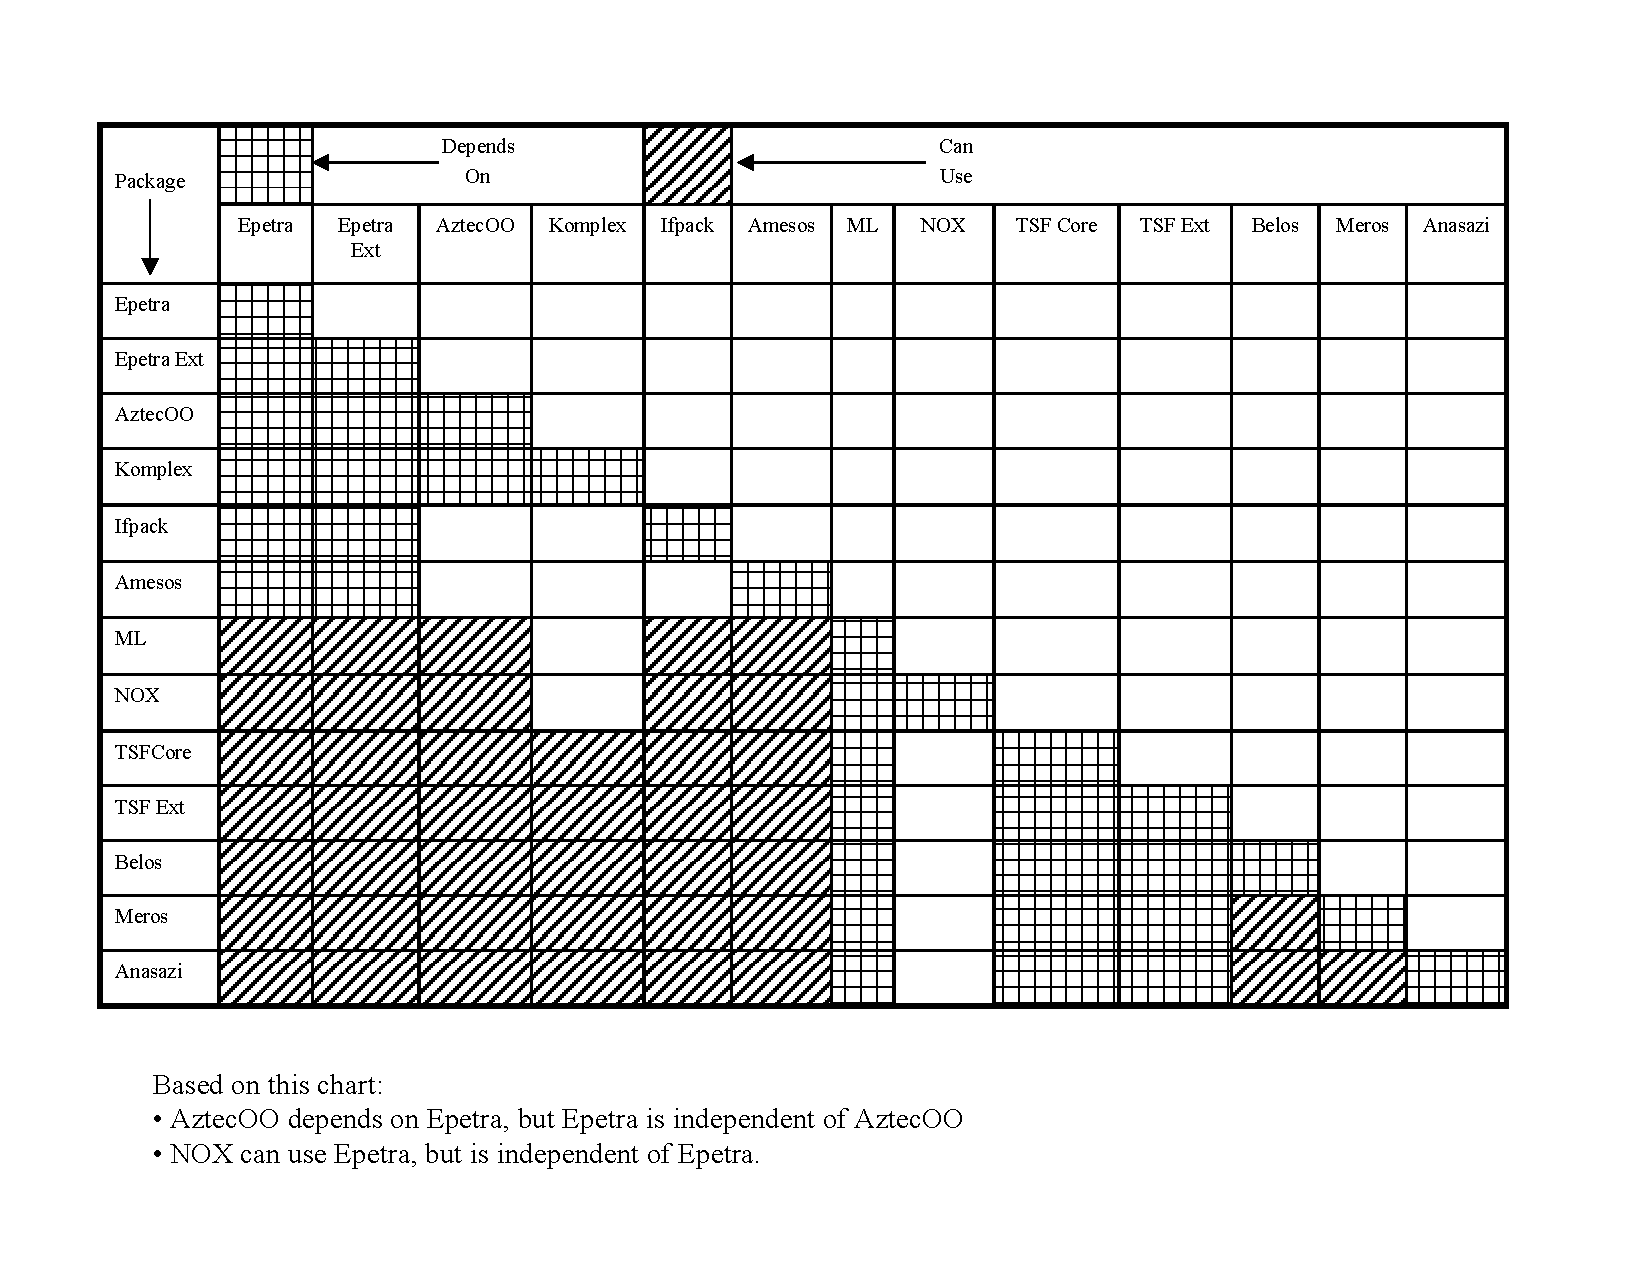
\includegraphics[height=6in,angle=270]{TrilinosPackageDependencies}
%\end{center}
\label{Figure:TrilinosPackageDependencies}
\caption{Current Trilinos Package Dependencies}
\end{figure}
collection of Trilinos packages depend on each other.

%\section{Platform Portablility}
%	**(List platforms - encourage script submission)**

\clearpage
\bibliographystyle{plain}
\bibliography{TrilinosDevGuide}
\addcontentsline{toc}{section}{References}

\appendix
\section{Commonly Used CVS Commands}
\label{Section:CVS}
\begin{itemize}

\item[Checking Out a Working Copy]

To get started, checkout a working copy of the development branch from the CVS 
repository.  (Releases branches can be obtained by by checking out the 
appropriate tagged version of the repository.  More about this below.)

\DisplayCommand{cvs checkout Trilinos}

\item[Updating a Working Copy]

To update after a version has been obtained use the \InlineCommand{cvs update} 
command.  First, cd to the directory that is to be updated (often the 
Trilinos root directory).  Then type:

\DisplayCommand{cvs -q update -dP}

The ``-q'' option means ``be somewhat quiet''.  Try an update without the 
``-q'' to see exactly what the option does.  

The ``-d'' option means to get any new directories.  For example, if a new 
package is added to the repository, but the ``-d'' option is not used, that 
new package will never appear in the working copy.  However, the first time 
that the ``-d'' option is used, all of the new package directories will be 
downloaded, and from that time on, all CVS updates will update the 
directories that were downloaded.  It is good practice to include this 
option for every CVS update.

Finally the ``-P'' option ``prunes'' empty directories.  This helps to keep 
the directory structure from getting more cluttered than it needs to.  For 
example, the old ``petra'' and ``tsf'' packages were removed from the 
repository, but the directory structures will remain if this option is not 
specified.  If an empty directory is needed, simply issue one update 
command without the ``-P'' and the empty directories will be restored.

\item{Viewing Local Changes}

After saving changes to a working copy of a branch of the Trilinos repository, 
the differences between the most recently obtained version of the edited 
file(s) and the current local version of the file(s) can be viewed using the 
following command:

\DisplayCommand{cvs -q diff}

The ``-q'' option again means ``be somewhat quiet''.  Try a diff without the 
``-q'' to see exactly what the option does.  

The diff command works recursively, but optionally accepts options that 
specify specific files and/or directories.  For example, to see the diff's 
associated only with a file in the current directory named 
\InlineDirectory{abc.cpp}, as well as all files located (recursively) in the 
relative directory \InlineDirectory'{examples}, type

\DisplayCommand{cvs -q diff abc.cpp examples}

%\item{Committing Changes}
%update!

%\item{Working with Branches}
%cvs status

%... Must be expanded, add info about when to check in, and which branch... also move much of the cvs stuff from the add/remove file section to here
\end{itemize}

\section{Common Bugzilla Tasks}
\label{Section:BugzillaTasks}


\end{document}
